%%%%%%%%%%%%%%%%%%%%%%%%%%%%%%%%%%%%%%%%%%%%%%%%%%%%%%%%%%%%%%%%%%%%%%%%%%%%%
%%% LaTeX-Rahmen fuer das Erstellen von Bachelorarbeiten
%%%%%%%%%%%%%%%%%%%%%%%%%%%%%%%%%%%%%%%%%%%%%%%%%%%%%%%%%%%%%%%%%%%%%%%%%%%%%

%%%%%%%%%%%%%%%%%%%%%%%%%%%%%%%%%%%%%%%%%%%%%%%%%%%%%%%%%%%%%%%%%%%%%%%%%%%%%
%%% allgemeine Einstellungen
%%%%%%%%%%%%%%%%%%%%%%%%%%%%%%%%%%%%%%%%%%%%%%%%%%%%%%%%%%%%%%%%%%%%%%%%%%%%%

\documentclass[twoside,12pt,a4paper]{report}
%\usepackage{reportpage}
\usepackage{epsf,german}
\usepackage{graphics, graphicx}
\usepackage[utf8]{inputenc}
\usepackage{float}
\usepackage{latexsym}
\usepackage[margin=10pt,font=small,labelfont=bf]{caption}
\usepackage{color} 
\usepackage{hyperref}
\setlength{\textfloatsep}{12pt}
\setlength{\intextsep}{12pt}
\setlength{\floatsep}{12pt}

\makeatletter
\setlength{\@fptop}{0pt}
\makeatother

\hypersetup{
    colorlinks=true, %set true if you want colored links
    linktoc=all,     %set to all if you want both sections and subsections linked
    linkcolor=black,  %choose some color if you want links to stand out
    citecolor=black,
    urlcolor=black,
}
\textwidth 14cm
\textheight 22cm
\topmargin 0.0cm
\evensidemargin 1cm
\oddsidemargin 1cm
%\footskip 2cm
\parskip0.5explus0.1exminus0.1ex

% Kann von Student auch nach pers\"onlichem Geschmack ver\"andert werden.
\pagestyle{headings}

\sloppy

\begin{document}

%%%%%%%%%%%%%%%%%%%%%%%%%%%%%%%%%%%%%%%%%%%%%%%%%%%%%%%%%%%%%%%%%%%%%%%%%%%%
%%% hier steht die neue Titelseite 
%%%%%%%%%%%%%%%%%%%%%%%%%%%%%%%%%%%%%%%%%%%%%%%%%%%%%%%%%%%%%%%%%%%%%%%%%%%%
 
\begin{titlepage}
 \begin{center}
  {\LARGE Eberhard Karls Universit"at T"ubingen}\\
  {\large Mathematisch-Naturwissenschaftliche Fakult"at \\
Wilhelm-Schickard-Institut f"ur Informatik\\[4cm]}
  {\huge Bachelorarbeit Informatik\\[2cm]}
  {\Large\bf Web-basierte Logik-Lehrtools mit React\\[1.5cm]}
 {\large Mike Hengge}\\[0.5cm]
15.03.2019\\[3cm]
\begin{center}{\small\bf Gutachter \& Betreuer}\\[0.5cm]
{\large Prof. Dr. Wolfang Küchlin}\\
  {\footnotesize Wilhelm-Schickard-Institut f\"ur Informatik\\
	Universit"at T"ubingen}	\end{center}
	
  \end{center}
\end{titlepage}

%%%%%%%%%%%%%%%%%%%%%%%%%%%%%%%%%%%%%%%%%%%%%%%%%%%%%%%%%%%%%%%%%%%%%%%%%%%%
%%% Titelr"uckseite: Bibliographische Angaben
%%%%%%%%%%%%%%%%%%%%%%%%%%%%%%%%%%%%%%%%%%%%%%%%%%%%%%%%%%%%%%%%%%%%%%%%%%%%

\thispagestyle{empty}
\vspace*{\fill}
\begin{minipage}{11.2cm}
\textbf{Hengge, Mike:}\\
\emph{Web-basierte Logik-Lehrtools mit React}\\ Bachelorarbeit Bioinformatik\\
Eberhard Karls Universit"at T"ubingen\\
Bearbeitungszeitraum: 15.11.2018-15.03.2019
\end{minipage}
\newpage

%%%%%%%%%%%%%%%%%%%%%%%%%%%%%%%%%%%%%%%%%%%%%%%%%%%%%%%%%%%%%%%%%%%%%%%%%%%%

\pagenumbering{roman}
\setcounter{page}{1}

%%%%%%%%%%%%%%%%%%%%%%%%%%%%%%%%%%%%%%%%%%%%%%%%%%%%%%%%%%%%%%%%%%%%%%%%%%%%%
%%% Inhaltsverzeichnis
%%%%%%%%%%%%%%%%%%%%%%%%%%%%%%%%%%%%%%%%%%%%%%%%%%%%%%%%%%%%%%%%%%%%%%%%%%%%%

\renewcommand{\baselinestretch}{1.3}
\small\normalsize

\tableofcontents

\renewcommand{\baselinestretch}{1}
\small\normalsize

\clearpage

%%%%%%%%%%%%%%%%%%%%%%%%%%%%%%%%%%%%%%%%%%%%%%%%%%%%%%%%%%%%%%%%%%%%%%%%%%%%%
%%% Abbildungsverzeichnis
%%%%%%%%%%%%%%%%%%%%%%%%%%%%%%%%%%%%%%%%%%%%%%%%%%%%%%%%%%%%%%%%%%%%%%%%%%%%%

\renewcommand{\baselinestretch}{1.3}
\small\normalsize

\addcontentsline{toc}{chapter}{Abbildungsverzeichnis}
\listoffigures

\renewcommand{\baselinestretch}{1}
\small\normalsize

\clearpage

%%%%%%%%%%%%%%%%%%%%%%%%%%%%%%%%%%%%%%%%%%%%%%%%%%%%%%%%%%%%%%%%%%%%%%%%%%%%%
%%% Der Haupttext, ab hier mit arabischer Numerierung
%%% Mit \input{dateiname} werden die Datei `dateiname' eingebunden
%%%%%%%%%%%%%%%%%%%%%%%%%%%%%%%%%%%%%%%%%%%%%%%%%%%%%%%%%%%%%%%%%%%%%%%%%%%%%

\pagenumbering{arabic}
\setcounter{page}{1}

%% Introduction
%%%%%%%%%%%%%%%%%%%%%%%%%%%%%%%%%%%%%%%%%%%%%%%%%%%%%%%%%%%%%%%%%%%%
% Einleitung
%%%%%%%%%%%%%%%%%%%%%%%%%%%%%%%%%%%%%%%%%%%%%%%%%%%%%%%%%%%%%%%%%%%%

\chapter{Einleitung}\label{Einleitung}
In den letzten Jahrzehnten hat sich das Internet über die ganze Welt verbreitet. Aktuell dient das Internet vielerorts als primäres Informations- und Kommunikationsmedium. Dabei wandelten sich die Ansprüche an dieses Medium mit dem technologischen Fortschritt. Mit leistungsfähigerer Hardware, sowohl auf Nutzer als auch auf Entwicklerseite, und schnelleren Internetverbindungen wurden neue Inhalte und neue Wege der Darstellung möglich.\\
Dank dieser neuen Möglichkeiten werden mehr und mehr Anwendungen über das Web angeboten, welche vorher nur als Desktopapplikationen zur Verfügung standen. Um solche Webapplikationen zu entwickeln werden oftmals spezielle JavaScript-Bibliotheken und -Frameworks verwendet. Beispiele sind Angular, Vue, React und noch viele mehr. React zeichnet sich dabei derzeit durch die größte Beliebheit aus.\\
React ist eine open-source JavaScript Bibliothek und wurde von Facebook entwickelt um möglichst performante Oberflächen zu gestalten. Seine Beliebtheit gründet sich auf der einfachen und schnellen Nutzung, mit hochperformanten Ergebnissen. Dabei beschränkt sich React auf den View-Teil der klassischen Model-View-Controller Struktur. Diese View besteht aus einzelnen Komponenten von denen jeder seinen eigenen 'State' verwaltet. Ändern sich diese States werden nur die betroffenen Komponenten neu gerendert, einer der Gründe für Reacts hohe Effizienz.\\\\
Die vorliegende Arbeit erfüllt zwei Funktionen und ist daher auch inhaltlich zweigeteilt. Zum einen sind in ihr Ergebnisse der Recherche und Evaluation von React aufgeführt. Zum Anderen beschäftigt sie sich mit der Umsetzung des im Folgenden beschriebenen Projekts. \\
Ziel des Recherche-Teils ist es, Reacts Eigenschaften, Vorteile, Nachteile und generelle Nutzbarkeit darzustellen. Dieser Teil soll dem Anspruch gerecht werden, eine fundierte Entscheidung für oder gegen eine eigene Nutzung von React zu ermöglichen. Anschließend werden gängige Komponenten der Entwicklung mit React vorgestellt. Dies stellt einen inhaltlichen Übergang in das praktische Projekt dar.\\\\
Bei dem Projekt handelt es sich um die Erstellung einer web-basierten Anwendung mittels JavaScript und React aus einer bestehenden stand-alone Java Implementierung „Logik Lehrtools“. In dieser werden in einer Nutzeroberfläche die Algorithmen Resolution, Backward Dual Resolution und Variablen-Elimination aus der Aussagenlogik auf dort eingegebene Formeln angewandt und die Zwischenergebnisse und Endergebnisse der Algorithmen ausgegeben. \\
Das entstehende Online-Tool soll für die Lehre einsetzbar sein und eine Möglichkeit für Studierende bieten Beispiele selbst nachzuvollziehen, den Ablauf der einzelnen Algorithmen zu beobachten und eigene Lösungen zu kontrollieren. Hierfür wird es nach Fertigstellung über einen Webserver im Universitätsnetzwerk zur Verfügung gestellt. 



\clearpage

%% 
%%%%%%%%%%%%%%%%%%%%%%%%%%%%%%%%%%%%%%%%%%%%%%%%%%%%%%%%%%%%%%%%%%%%
% Diskussion und Ausblick
%%%%%%%%%%%%%%%%%%%%%%%%%%%%%%%%%%%%%%%%%%%%%%%%%%%%%%%%%%%%%%%%%%%%

\chapter{React - Theorie und Evaluation}
  \label{Evalution React}

\section{Motivation}
React wurde 2013 von Facebook entwickelt. Seine Entstehung ist direkt verknüpft mit den Problemen von JavaScript, die speziell bei großen Anwendungen auftreten. Das von JavaScript verwendete DOM ist bei oftmaligen Zustandsänderungen langsam und ineffizient. Durch den Aufbau des DOM muss dieses auch bei kleinen Änderungen in Gänze neu geladen werden. Es gilt außerdem allgemein als fehleranfällig, unnötig kompliziert und ist für die Webentwicklung nicht sehr gut geeignet. \cite{2}\\
Hinzu kommt, dass JavaScript-Objekte nicht funktional sind, das heißt ihr Zustand ist nicht nur vom Input und darauf ausgeführten Funktionen abhängig. Stattdessen teilen sich Objekte oftmals Zustände und verändern sich so mitunter gegenseitig. Daher war Frontendcode vor React oft unverständlich und schwer wartbar. \cite{2}\\
Das Ziel der Entwicklung Reacts war es deswegen weniger komplexen und gut lesbaren Code zu ermöglichen, der Zustände persistent und effizient verwaltet \cite{3}. Die sonst oft in der Webentwicklung verwendeten Templates sollten ersetzt werden. Stattdessen sollte eine Lösung die mehr Flexibilität bietet und es gleichzeitig durch kompaktere Architektur erleichtert Applikationen auszuweiten eingeführt werden \cite{1}.
\section{Architektur}
Im Vergleich zu den bis dato gängigen JavaScript Frameworks und JavaScript selbst, weist React einige Besonderheiten in seiner Architektur auf. Die wichtigsten dieser Besonderheiten werden hier im Folgenden aufgeführt und diskutiert. Es gibt noch einige weitere Eigenheiten Reacts, doch diese vier sind die ausschlaggebenden Merkmale für dessen Erfolg und stehen deshalb im Fokus dieser Evaluation.
\subsection{Virtual DOM}
In der Webentwicklung hat die Manipulation des Document Object Model (DOM) eine ausschlaggebende Rolle inne. Mit ihr kann der Elementbaum einer Webseite ausgelesen, verändert und erweitert werden. Wie oben erwähnt ist das JavaScript DOM problematisch.\\
React löst dieses Problem mittels dem sogenannten Virtual DOM, welche ein entsprechendes virtuelles Model des eigentlichen DOMs ist \cite{4}. Jedes DOM-Objekt wird darin über ein ähnliches oder vereinfachtes virtuelles Objekt dargestellt. Obwohl es in seinen Eigenschaften dem DOM stark ähnelt, kann das virtuelle DOM keine direkten Änderungen am Elementbaum durchführen. Stattdessen wird seine erheblich bessere Performanz als Änderungsbuffer benutzt. Wird ein React Komponent (siehe 2.3) gerendert, so wird ein Snapshot des aktuellen Zustands gemacht und alle virtuellen DOM-Objekte werden aktualisiert. Dieser Prozess ist weitaus schneller als das Aktualisieren des eigenlichen DOM, da keine tatsächlich angezeigten Elemente verändert werden. Dabei beeinflusst er die Performanz des restlichen Systems nicht. Nachdem so alle virtuellen DOM-Objekte aktualisiert wurden, werden diese mittels dem sogennanten 'Diffing' mit dem Snapshot verglichen. Lediglich der Zustand der Objekte der sich zwischen diesen Schritten verändert hat, wird vom virtuellen DOM in das DOM übernommen \cite{3}. In Abbildung 2.1 ist dieser Prozess in einem Schaubild dargestellt.\\
\begin{figure}[H]
     \centerline{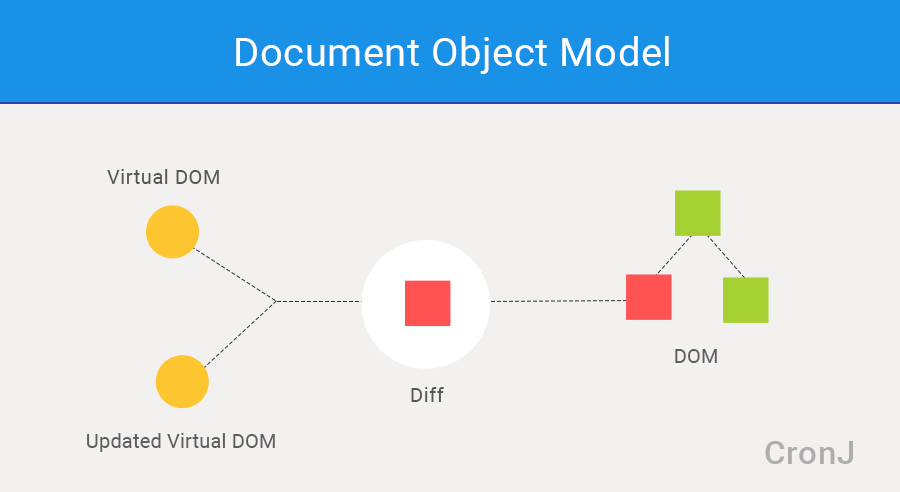
\includegraphics[width=14cm]{../Abbildungen/virtualDom.png}}
  \caption{React Virtual DOM \cite{Abb2.1}}
  \label{React Virtual DOM}
\end{figure}
\noindent Resultat ist eine erheblich schnellere, effizientere und performantere DOM-Manipulation als frühere Lösungen. Das Virtual DOM kann fraglos als einer der Hauptgründe für Reacts Beliebtheit bezeichnet werden.
\subsection{Komponenten}
Komponenten sind die wichtigsten Bausteine einer React Anwendung. Sie sind vergleichbar mit JavaScript Klassen und Funktionen. Mit sogenannten Props (Properties) als Input liefern Komponenten React-Elemente an die View. So legen sie das Aussehen eines Teils der Benutzeroberfläche fest, deren Gesamtheit aus vielen verschachtelten Komponenten besteht. Ein Beispiel einer simplen 'Hello World'-Komponente in React ist in Abbildung 2.2 abgebildet.
\begin{figure}[H]
     \centerline{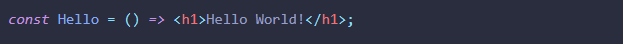
\includegraphics[width=12cm]{../Abbildungen/compHello.png}}
  \caption{Hello World Komponente \cite{eig}}
  \label{Hello World Komponente}
\end{figure}
Komponenten sind wiederverwendbar und veränderbar. Durch die Implementierung von Komponenten besteht die Benutzeroberfläche in React aus diesen vielen kleinen Elementen des gleichen Typs und ist dadurch leicht anzupassen, nachzuvollziehen und zu testen. Sind Änderungen an einer bestimmten Komponente nötig, so kann direkt auf diese zugegriffen und ihr Inhalt verändert werden. Am Beispiel in Abbildung 2.3 die dem React-Lehrbuch 'Learning React' entnommen ist, ist dies gut zu erkennen. Hier markiert jeder der rechteckigen Ränder eine Komponente. Wäre es nötig die Zubereitung des 'Curried Egg Salad' zu ändern, ist dies problemlos möglich da es eine eigene Komponente ist. So ist kein Zugriff auf andere Komponenten nötig und es wird eine versehentliche Änderung dieser ausgeschlossen.\\
\begin{figure}[H]
     \centerline{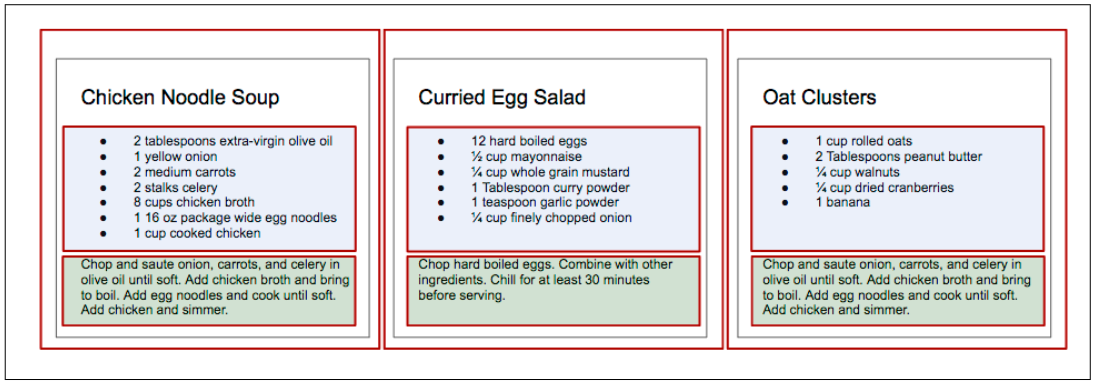
\includegraphics[width=12cm]{../Abbildungen/compContainer.png}}
  \caption{Hello World Komponente \cite{6}}
  \label{Hello World Komponente}
\end{figure}
\clearpage
\subsection{Unidirektionaler Datenfluss}
Anders als viele der beliebten Frameworks verwendet React keinen bidirektionalen Datenfluss. Ebenso erstellt es in dem bekannten Model-View-Controller Konzept nur die View-Komponente und überlässt dem Entwickler die Wahl, ob und welche weiteren Komponenten verwendet werden \cite{5}. In einem bidirektionalen Datenfluss sind Model und View in direktem, gegenseitigem Austausch \cite{5}. In diesem Austausch lösen Änderungen an einer Seite entsprechende Änderungen auf der anderen Seite aus. Diese gängige Lösung wird in den meisten Fällen gute Leistungen und Ergebnisse erzielen. Jedoch können unvorhersehbaren Datenflüsse auftreten, eben weil sowohl Model als auch View Einfluss auf den Zustand der Anwendung haben. Es kann so zu nicht beabsichtigten Änderungen in nicht bearbeiteten Model-Bereichen und zu Kettenreaktionen von Updates kommen.\\
In React können Daten stattdessen nur in eine Richtung gegeben und verarbeitet werden, React ist also unidirektional. So wird ein Jonglieren der Zustände vermieden. \\
\begin{figure}[H]
     \centerline{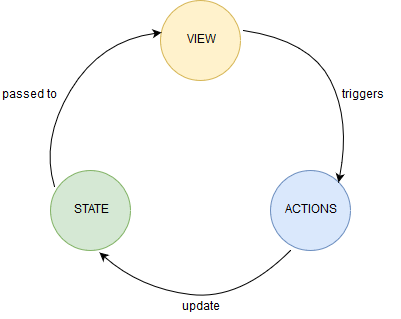
\includegraphics[width=12cm]{../Abbildungen/dataflow.png}}
  \caption{Unidirektionaler Datenfluss in React \cite{eig}}
  \label{Unidirektionaler Datenfluss in React}
\end{figure}
\clearpage \noindent In Abbildung 2.4 ist zu sehen, wie die Daten hier in einem Kreislauf durch Zustand, View und Aktionen fließen. Der Anwendungszustand, der die Zustände der Komponenten beinhaltet, wird an die View und ihre Child-Komponenten weitergegeben. In dieser werden Aktionen getriggered, beispielsweise durch den Nutzer, welche den Zustand verändern können. \\
Wie in Punkt 2.1 erwähnt, konnte es vor React oftmals schwierig sein den Datenfluss in einer Anwendung nachzuverfolgen. Der unidirektionale Datenfluss Reacts schafft hier eine größere Nachvollziehbarkeit und begünstigt so Analyse und Fehlersuche. \\
\subsection{JSX}
JSX ist eine Syntax-Erweiterung zu JavaScript die für React empfehlenswert ist, da sie durch ihre Ähnlichkeit mit HTML-Syntax leicht zu lesen und zu verwenden ist \cite{5}. Der Typ eines Elements wird wie in HTML in einem öffnenden Tag festgelegt. Zwischen diesem öffnendem und dem nachfolgenden schließendem Tag können die Kinder des Elements hinzugefügt werden. In Abbildung 2.5 ist als Beispiel eine ungeordnete Liste in JSX dargestellt.
\begin{figure}[!thb]
     \centerline{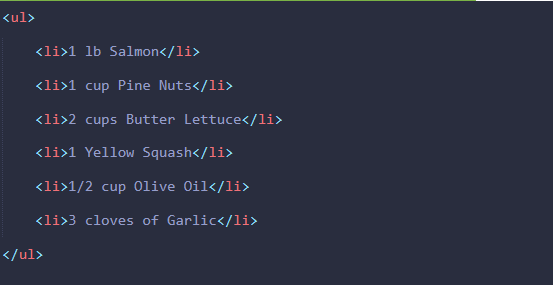
\includegraphics[width=12cm]{../Abbildungen/jsxList.png}}
  \caption{Ungeordnete Liste in JSX \cite{eig}}
  \label{Ungeordnete Liste in JSX}
\end{figure}
In JSX werden JavaScript-Ausdrücke in geschweifte Klammern gestellt. Die Anzeige des Titel-Felds eines Elements wäre beispielsweise wie in Abbildung 2.6 umzusetzen.\\ 
\begin{figure}[H]
     \centerline{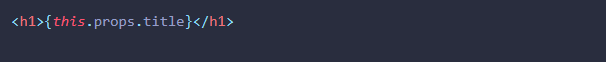
\includegraphics[width=12cm]{../Abbildungen/jsxExpression.png}}
  \caption{JavaScript in JSX \cite{eig}}
  \label{JavaScript in JSX}
  \centerline{}
     \centerline{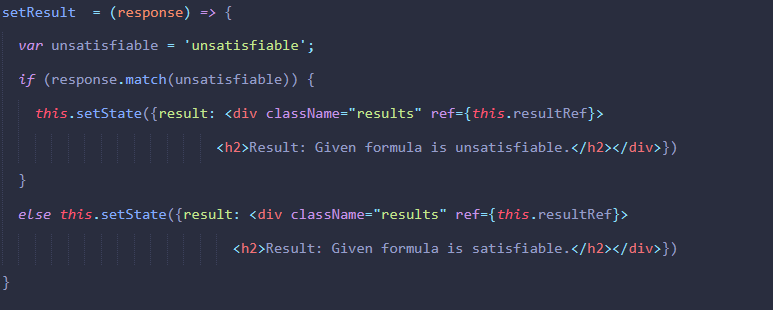
\includegraphics[width=12cm]{../Abbildungen/jsxSetResult.png}}
  \caption{Funktion setResult in JSX \cite{eig}}
  \label{Funktion setResult in JSX}
\end{figure}
\noindent Die Ausdrücke werden als vollwertiges Skript ausgeführt, es ist daher auch möglich vorher definierte Funktionen und vorimplementierte JavaScript Operationen an dieser Stelle zu verwenden. Da JSX eine Erweiterung zu JavaScript ist, kann in derartigen Funktionen auch JSX-Syntax verwendet werden. Wie in Abbildung 2.7 gezeigt, könnte beispielsweise eine Funktion setResult erstellt werden, die einen erhaltenen String untersucht und abhängig von dessen Inhalt zwei unterschiedliche JSX-Sequenzen ausgibt. \\
JSX bietet einige Vorteile gegenüber dem üblichen JavaScript. Da JSX-Code während er zu JavaScript kompiliert automatisch optimiert wird, sind Anwendungen in JSX mindestens gleich schnell wie equivalente Anwendungen in JavaScript. Dieses Kompilieren fängt außerdem Fehler ab und erhöht so die Qualität der Anwendung. Diese Wirkung wird noch verstärkt durch die zusätzlichen Debugging Möglichkeiten die JSX auf Compiler Level bietet. Dank der Syntax die HTML und JavaScript vereint, ist JSX sehr leicht zugänglich und benötigt wenig Einarbeitungszeit. \\
Als interpretierte Programmiersprache wird JavaScript üblicherweise ohne vorherigen Kompilierschritt vom Browser gelesen und interpretiert. Da Browser aber JSX nicht erkennen, ist Kompilieren hier notwendig. Dieser Prozess wird auch Transpiling genannt. Üblich ist hier die Nutzung des Babel-Projekts, welches auch von den großen React-Nutzern Facebook, PayPal, Netflix und AirBnB genutzt wird und welches schon über einen kurzen Import genutzt werden kann \cite{6}. Da die Verwendung von Toolchains (siehe Punkt 3.1.2) diese Konfiguration automatisch übernimmt, ist es jedoch sehr selten nötig dies selbst zu tun.\\
\section{Stärken}
Wie in den Passagen oben zu sehen, gibt es gute Gründe warum React so schnell so beliebt wurde. Als Bibliothek für JavaScript ist React ein Teil der beliebtesten Programmiersprache für Webseiten der Welt und verbessert diese an den nötigen Stellen. Reacts virtuelle DOM ist schnell, effizient und dynamisch und so der JavaScript DOM überlegen. Der unidirektionale Datenfluss bietet als neuer Ansatz ebenso einige Vorteile gegenüber dem bidirektionalen Fluss anderer Frameworks. Durch diese Besonderheiten seiner Architektur ist es auch für große Webanwendungen gut geeignet. Besonders die Fehleranfälligkeit und Unsicherheit JavaScripts konnte verbessert werden \cite{6}.\\
Mit der JSX-Syntax und der Nähe zur funktionalen Programmierung sind React Anwendungen intuitiv, übersichtlich, gut testbar und bieten eine gute Performanz. Da React dem Entwickler als Bibliothek weniger Einschränkungen auferlegt als es Frameworks gewöhnlich tun, ist es sehr leicht auf das große JavaScript Toolset zuzugreifen und zusätzliche Werkzeuge, Programme und Pakete in die Anwendung einzubinden.\cite{6} \\
Da React als Projekt fast von Beginn an Open Source war, gut dokumentiert ist und die genannten Vorteile bietet, besitzt es mittlerweile eine sehr aktive Gemeinschaft. Es wird ständig weiterentwickelt und bietet immer mehr Funktionen an. Entwickler stehen mit Problemen, Lösungen und Fragen in stetem Austausch. React bietet daher eine gute Lernumgebung, in der es leicht ist Lösungen bei bekannten und Hilfe bei unbekannten Problemen zu finden.\\
\section{Kritik}
Die ständige Weiterentwicklung von React ist aber auch ein oft genannter Kritikpunkt, wie die Webrecherche zeigt \cite{7}. Es entstehen so schnell neue Bibliotheken und Tools, dass es gerade bei großen Projekten schwer sein kann, die am besten passende Umgebung zu finden. Ständiges Lernen und tiefes Verständnis der Technologie ist nötig um stets die Aktuellsten dieser Werkzeuge verwenden zu können. Die große Bandbreite kann es schwer machen sich auf eine Lösung festzulegen. \\
Da React nur die View-Komponente bedient, ist es gerade bei größeren Anwendungen oft nicht möglich, ausschließlich React zu verwenden. So ist es beispielsweise für eine große Anwendung sehr zeitaufwendig und kompliziert die Zustände aller Komponenten zu verwalten. Es ist daher hilfreich einen Zustandsmanager wie Flux oder Redux zu verwenden \cite{5}. Ein solcher Manager bringt aber seine eigene Architektur mit, die verstanden und korrekt verwendet werden muss. Sollen Einstellungen am Routing verfübar sein, muss React-Router installiert werden. Werden Tests gebraucht, so installiert man für Unit Testing Jest oder Enzyme, für Integration Testing Karma oder für E2E Testing Selenium. Es existiert für fast alle Anforderungen mindestens eine gute Lösung, aber in sehr wenigen Fällen ist diese schon in React enthalten. Bei der Suche nach dieser Lösung ist es dann oft schwer eine fundierte Entscheidung für oder gegen eine der Möglichkeiten zu treffen. \\
Während es für kleine Projekte noch möglich ist die Umgebung selbst aufzubauen, ist dies für größere zu komplex und zeitaufwendig. So ist man angewiesen auf Toolchains (siehe 3.1.2), bei deren Vielzahl die Suche nach der passenden ebenfalls schwer sein kann. \\
Zusammenfassend ist React durch ständige Veränderungen und Erweiterungen schwer zu meistern. So ist React zwar intuitiv und übersichtlich, doch die Abhängigkeit von Verständnis und stetigem Lernen gibt dennoch eine stetig steile Lernkurve. 

\section{Alternativen}
Viele der Verbesserungen die React enthält wurden seitdem auch in anderen JavaScript-Frameworks und -Bibliotheken umgesetzt. Diese Passage beschränkt sich mit Ausnahme Angulars auf solche Projekte. Es werden die Frameworks Angular und Vue und die Bibliotheken Preact und Riot im Vergleich zu React vorgestellt.\\
\subsection{Angular}
Angular ist ein JavaScript-Framework welches seit 2009 von Google entwickelt wird und ebenfalls kostenlos zur Verfügung steht. Im Gegensatz zu React implementiert Angular das ganze Model-View-Controller-Architekturmuster, verwendet bidirektionale Datenflüsse und manipuliert das DOM direkt \cite{5}. Statt JSX ist TypeScript die empfohlene Syntax. Abhängigkeiten werden automatisch verwaltet, es sind also keine Toolchains oder manuelle Verwaltung nötig.\\
Obwohl Angular ein Framework und React eine Bibliothek ist, unterscheidet sich die Anwendung kaum. Beide werden für die Frontend-Entwicklung verwendet. Als relativ altes Framework implementiert Angular aber viele Technologien, die in React gezielt vermieden oder verbessert wurden. Dennoch ist Angular wettbewerbsfähig, vor allem da es als Framework ohne weitere Bibliotheken auskommt und so weniger Entscheidungen während dem Projekt nötig sind. Ebenso kann dadurch jedoch unter Umständen eine viel zu große Anzahl an Funktionen vorhanden sein, die nicht benötigt werden.
\subsection{Vue}
Das ebenfalls kostenlose Framework Vue ähnelt React sehr viel mehr als es Angular tut. Es erschien 2014 und griff viele von Reacts Neuerungen auf. Wie React verwendet auch Vue eine virtuelle DOM, arbeitet mit View-Komponenten und beschränkt sich auf eine schmale Kernbibliothek \cite{8}. Genau wie in React werden auch in Vue Zusatzfunktionen oft nur durch die Installation von weiteren Tools angeboten. Obwohl Vue auch JSX unterstützt, sind Templates in diesem Framework die empfohlene Methode eine Anwendung aufzubauen. Vue ähnelt darin vielen anderen Frameworks und bietet so bekannte Elemente für viele Entwickler. \\
Ein wichtiger Unterschied besteht bei der Auswahl von zusätzlichen Tools, sogennanten Companion Libraries. Während diese in React ohne Kontrolle von Entwicklern aus der Gemeinschaft zur Verfügung gestellt werden, werden sie von Vue offiziell unterstützt und zusammen mit der Kernbibliothek aktualisiert. So gibt es zwar in React weit mehr Möglichkeiten, doch sind diese verstreut und unübersichtlich. \cite{8}\\
Des Weiteren bietet Vue eine bessere Möglichkeit zur automatischen Konfiguration von Projekten. Die erwähnten Toolchains für React sind vielfältig und hilfreich, doch bieten sie während dem Prozess wenig Konfigurationsmöglichkeiten. Mit Vues 'ClI project generator' sind dagegen zahlreiche solcher Möglichkeiten geboten. \cite{8} \\\\
Angular ist die 'klassische' Alternative zu React und kann für Projekte aller Art verwendet werden.
\begin{figure}[!thb]
     \centerline{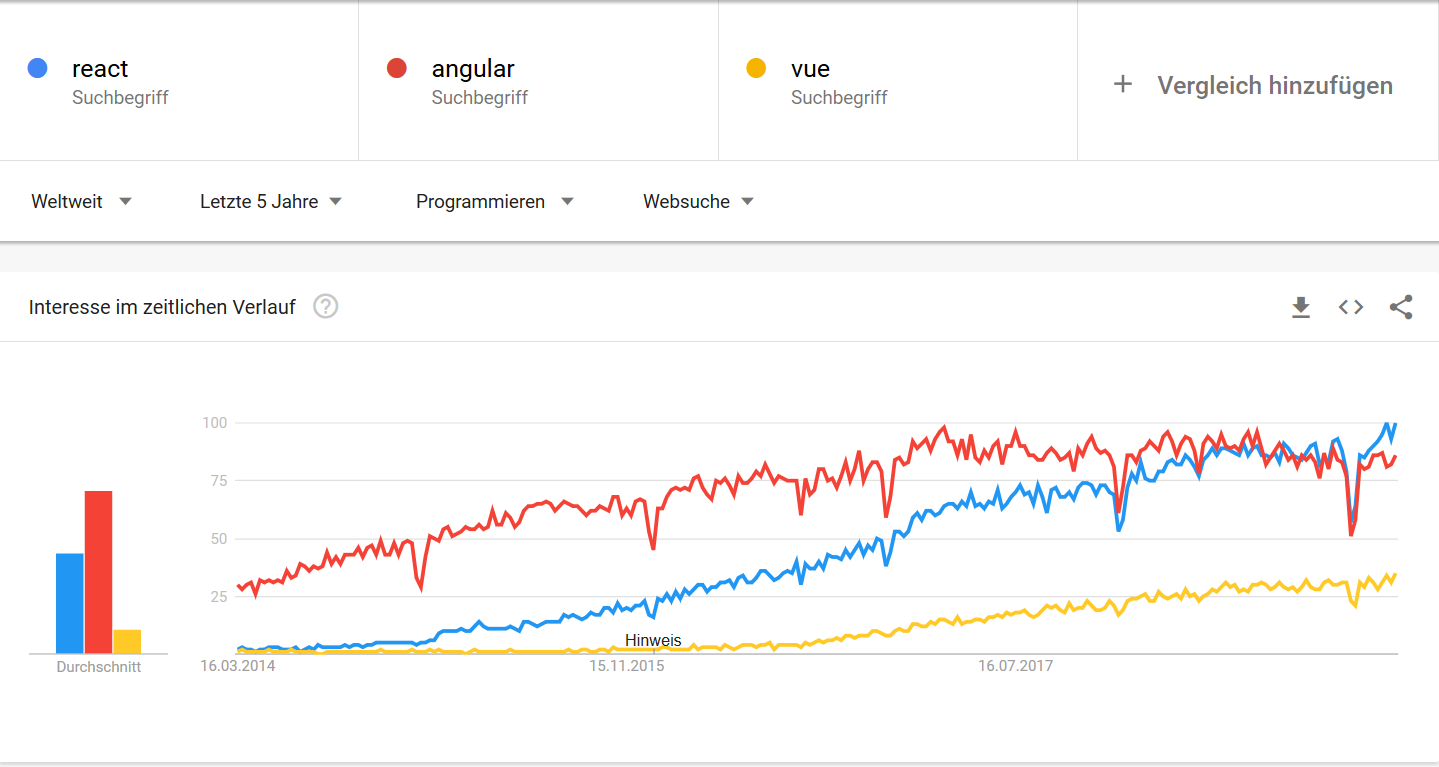
\includegraphics[width=12cm]{../Abbildungen/reactVueAng.png}}
  \caption{Trend der Suchanfragen seit 2014 für React, Angular und Vue \cite{Abb2.8}}
  \label{Trend der Suchanfragen}
\end{figure}
Neben Angular ist Vue Reacts größter Konkurrent. In Abbildung 2.8 ist der Verlauf von Google-Suchanfragen der letzten fünf Jahre, als Indikator der Beliebheit der drei Lösungen, dargestellt. Wie deutlich zu sehen ist, hat React in den letzten Jahren auf Angular aufgeschlossen und es nun sogar überholt. Vue dagegen war lange Zeit kaum bekannt und begann erst in den letzten beiden Jahren aufzuholen.\\\\ 
Vue kann als vielversprechende Alternative zu React gesehen werden. Besonders für Webentwickler die Templates gewohnt sind und sich keine neue Syntax aneignen wollen ist es sehr gut geeignet. In Performanz und Funktionalität ist Vue nahezu gleichwertig zu React und bietet die oben genannten Besonderheiten.
\subsection{Preact}
Preact ist eine sehr kleine Alternative zu React. Die Bibliothek ist nur 3kB groß und damit etwa 15-mal kleiner als React. Preact vereinfacht und entfernt dabei manche Funktionalitäten von React und hat besonders beim Diffing (Feststellen der Änderungen an dem virtuellen DOM) kleinere und schnellere Lösungen \cite{9}. Hinzu kommt, dass in Preact effizientes Recycling von DOM-Elementen betreibt und dadurch zusätzlich Zeit einspart. \\
Die Bibliothek bietet so eine schnellere, kleinere Lösung, besitzt aber weniger Funktionen. Da es derzeit relativ unbekannt ist, sind weit weniger ergänzende Tools für Preact vorhanden. \\\\
Preact kann also besonders für kleine Projekte eine einfachere Alternative zu React darstellen.
\subsection{Riot}
Auch Riot ist, laut dessen Entwicklern, direkt von React inspiriert. Die Bibliothek verfügt aber über eine eigene, knappere Syntax und, wie Preact, über einen vereinfachten Algorithmus für das Diffing. Außerdem sind sowohl ein Routing- als auch ein State-Management-Tool eingebaut. Diese beiden Werkzeuge müssen in React oft noch während dem Projekt implementiert werden.\\
Riot hat nur ein Viertel von Reacts Größe und bietet dennoch große Funktionalität an. Auch diese Lösung ist aber noch relativ unbekannt und weist so langsamere Entwicklung und weniger Tools auf.\\\\
Für Riot gilt daher ähnliches wie für Preact. Besonders für kleine Projekte ist es eine sehr gute Alternative zu React, doch muss es noch an Beliebtheit gewinnen.
\section{Fazit}
React ist eine sehr mächtige und sehr praktische Bibliothek. Die Verbesserungen die es gegenüber früheren Frameworks mit sich brachte waren wegweisend, haben sich durchgesetzt und viele neue Projekte inspiriert. Es bietet zahlreiche Möglichkeiten, Tools und Erweiterungen und kann so jede Anforderung bedienen. Meiner Meinung nach gibt es sogar im Unternehmensbereich wenige Anforderungen denen React nicht gerecht werden kann. \\
Natürlich hat aber auch React, wie oben aufgeführt, Bereiche die verbesserungswürdig sind. Andere Projekte wie Vue, die diese Probleme scheinbar besser gelöst haben, sind bereits auf dem Markt und bieten starke Alternativen. Während React sich momentan dieser großen Beliebheit erfreut, gibt es daher aber auch starke Kritik an der Bibliothek. Bei der großen Geschwindigkeit mit der der Bereich Frontend-Entwicklung wächst, ist es schwer vorauszusagen wie lange React noch so beliebt bleiben wird. \\\\
Diese Sachverhalte führen zu folgender Schlussfolgerung: Momentan ist es definitiv nicht falsch sich für React zu entscheiden. Wie schnell sich das ändert ist aber nicht absehbar. 
\clearpage

%%
%%%%%%%%%%%%%%%%%%%%%%%%%%%%%%%%%%%%%%%%%%%%%%%%%%%%%%%%%%%%%%%%%%%%
% Diskussion und Ausblick
%%%%%%%%%%%%%%%%%%%%%%%%%%%%%%%%%%%%%%%%%%%%%%%%%%%%%%%%%%%%%%%%%%%%

\chapter{React in der Praxis}
  \label{React in der Praxis}
\section{Entwicklungsumgebung}
\subsection{Nodejs}
Nodejs ist ein JavaScript Runtime Environment für die serverseitige Entwicklung mit JavaScript. Für Projekte mit React ist es vor allem wegen dem enthaltenen Paketmanager NPM wichtig. Dieser ist aktuell de-facto Standard zur Verteilung von Paketen in JavaScript und bietet die Möglichkeit die React-Applikation während der Entwicklung direkt über einen integrierten Webserver anzuzeigen. Ein weiterer wichtiger Vorteil von NPM ist die einfache Installation vieler Erweiterungsmodule, die spezielle Funktionen bieten und häufige Problemstellungen lösen können. \\
Der oben erwähnte Webserver ist die einfachste Möglichkeit eine React-Applikation außerhalb einer Produktionsumgebung anzuzeigen. Anders als bei statischen Webseiten ohne Skriptanteil, können dynamische Webseiten nicht ohne eine Server-Client-Umgebung aufgerufen werden. Grund dafür ist, dass der dynamische Inhalt erst beim Aufruf vom Server generiert wird. Soll die React-Applikation so angezeigt werden reicht dank NPM der kurze Befehl 'npm run start' um den Webserver zu starten und die Applikation anzuzeigen. Veränderungen im Code der Applikation werden dabei live kompiliert, was die Fehlersuche und das Testen neuer Komponenten stark erleichtert. Wie in Abbildung 4.1 zu sehen ist, steht die Applikation unter einen lokalen URL zur Verfügung und könnte durch einen weiteren kurzen befehl 'npm run build' für die Produktion optimiert werden.
\begin{figure}[H]
     \centerline{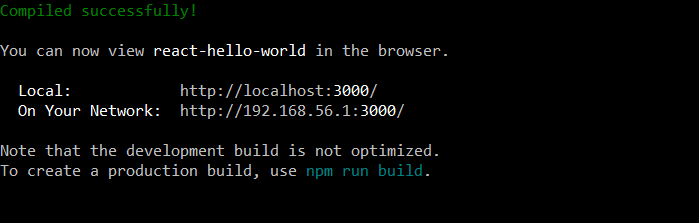
\includegraphics[width=14cm]{../Abbildungen/npmRunStart.png}}
  \caption{NPM Dialog}
  \label{NPM Dialog}
\end{figure}
\subsection{Toolchains für React}
Für React sind eine Vielzahl von Toolchains zur Vereinfachung der Entwicklung verfügbar. Diese stellen dem Entwickler eine fertige Umgebung zur Verfügung, die entsprechende Abhängigkeiten und Tools beinhaltet.Während es problemlos möglich ist ohne diese Werkzeugprogramme eine React Applikation zu entwickeln, sind sie in bestimmten Fällen sehr empfehlenswert. Besonders bei sehr großen Projekten mit vielen Komponenten und zusätzlichen Tools sind entsprechende Toolchains wertvoll. Andere Vorteile sind die Vermeidung typischer Fehler im Projektaufbau und eine einfache Optimierung des Projekts für die Produktion.\\
Bekannte Toolchains sind unter anderem Create React App, Next.js und Gatsby. Create React App ist für die Entwicklung von single-page Applikationen wie dem LogikLehrtool-Projekt sehr gut geeignet. Next.js dagegen wird eher für die Entwicklung von serverseitig gerenderten Webseiten und Gatsby für statische Seiten verwendet. Darüber hinaus gibt es eine Vielzahl an weiteren Toolchains die sehr viele Anwendungsgebiete abdecken und auch für ungewöhnlichere Projekte eine passende Konfiguration erzeugen können.
\pagebreak
\section{React in HTML-Seiten einfügen}
Es ist recht einfach React einer bestehenden HTML-Seite hinzuzufügen. Im folgenden Beispiel wird in eine HTML-Seite ein Like-Button eingefügt.\\
\begin{figure}[thb]
     \centerline{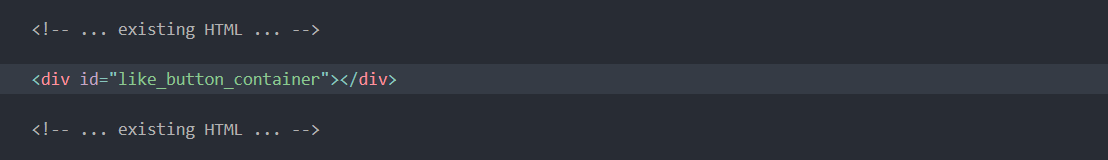
\includegraphics[width=14cm]{../Abbildungen/domContainer.png}}
  \caption{Erstellen eines Dom-Containers}
  \label{fig1_1}
  \vspace{1cm}
     \centerline{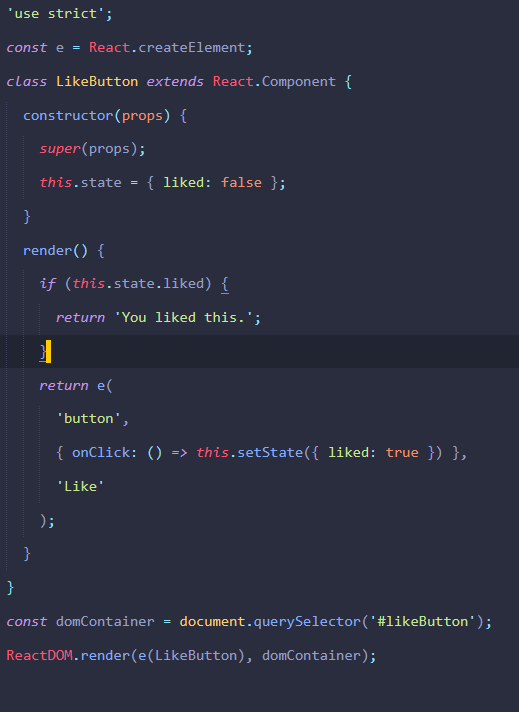
\includegraphics[width=8cm]{../Abbildungen/buttonScript.png}}
  \caption{Button.js: React-Script zur Verwendung des Dom-Containers}
  \label{fig1_1}
\end{figure}\\
Wie in Abbildung 4.1 zu sehen ist, wird als Erstes ein Dom-Container in der HTML-Datei eingefügt. Dieser Container wird anschließend bei der Erstellung eines React-Scripts mittels seiner ID verwendet. Abbildung 4.2 zeigt dieses Script, welches einen Button mit einer Klick-Reaktion erzeugt. Wird der Button geklickt, so ändert sich sein Status und es wird stattdessen der Satz 'You liked this' angezeigt. \\
Abschließend müssen in der HTML-Datei, wie in Abbildung 4.3, nur noch die entsprechenden Skripte geladen werden. Dies beinhaltet zwei Skripte, welche die React-Bibliothek laden und das eben erstellte Button-Skript, das die React-Komponente beinhaltet.
\begin{figure}[thb]
     \centerline{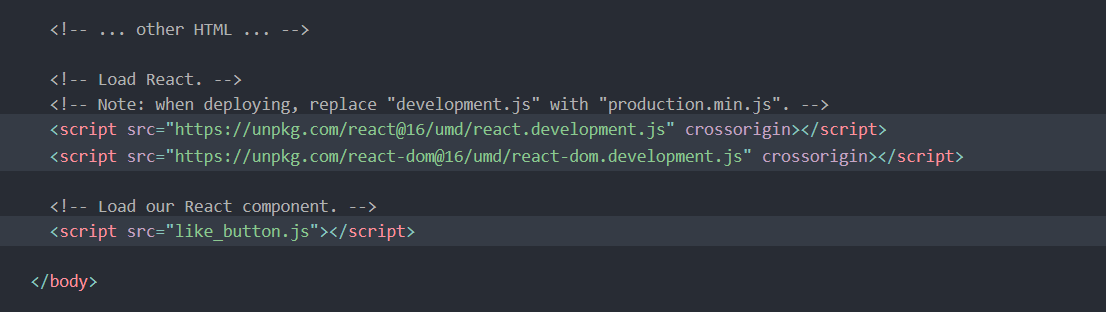
\includegraphics[width=14cm]{../Abbildungen/scriptLines.png}}
  \caption{Laden von React (Zeile 4+5) \& Button.js (Zeile 7)}
  \label{fig1_1}
\end{figure}\\

\clearpage

%%%%%%%%%%%%%%%%%%%%%%%%%%%%%%%%%%%%%%%%%%%%%%%%%%%%%%%%%%%%%%%%%%%%
% Diskussion und Ausblick
%%%%%%%%%%%%%%%%%%%%%%%%%%%%%%%%%%%%%%%%%%%%%%%%%%%%%%%%%%%%%%%%%%%%

\chapter{Logik Lehrtools mit React}\label{Lehrtools}
Dieses Kapitel beinhaltet den eingangs erwähnten zweiten Teil dieser Arbeit, das Logik-Lehrtools-Projekt. Dieser zweite Teil ist aufgeteilt in die Teilaufgaben die das Projekt mit sich brachte. Zunächst wird über ein Ablaufdiagramm gezeigt wann die einzelnen Komponenten bei der Nutzung zusammenspielen. Anschließend werden diese Komponenten detailliert aufgeführt. Dabei werden sowohl ihre Rolle im Ablauf, als auch Entscheidungen und Probleme der Projektdurchführung erläutert. Zuerst werden hier die durchgeführten Anpassungen am bereits vorhandenen Java-Programm vorgelegt und erklärt. Anschließend folgen die zwei Webentwicklungskomponenten: der verwendete Webserver und die React-Applikation. Abschließend dann die Server-Schnittstelle, die die Kommunikation zwischen Webseite und Java-Programm regelt.
\pagebreak
\section{Ablauf}
In Abbildung 4 ist der Ablauf vom Aufruf der Seite bis zur Anzeige der Resultate dargestellt. Deutlich sichtbar ist, wie nach den ersten beiden Schritten die Kommunikation nicht mehr über den Webserver abläuft. Stattdessen wird die neben dem Server laufende API nunmehr zentral für den Austausch.
\begin{figure}[H]
     \centerline{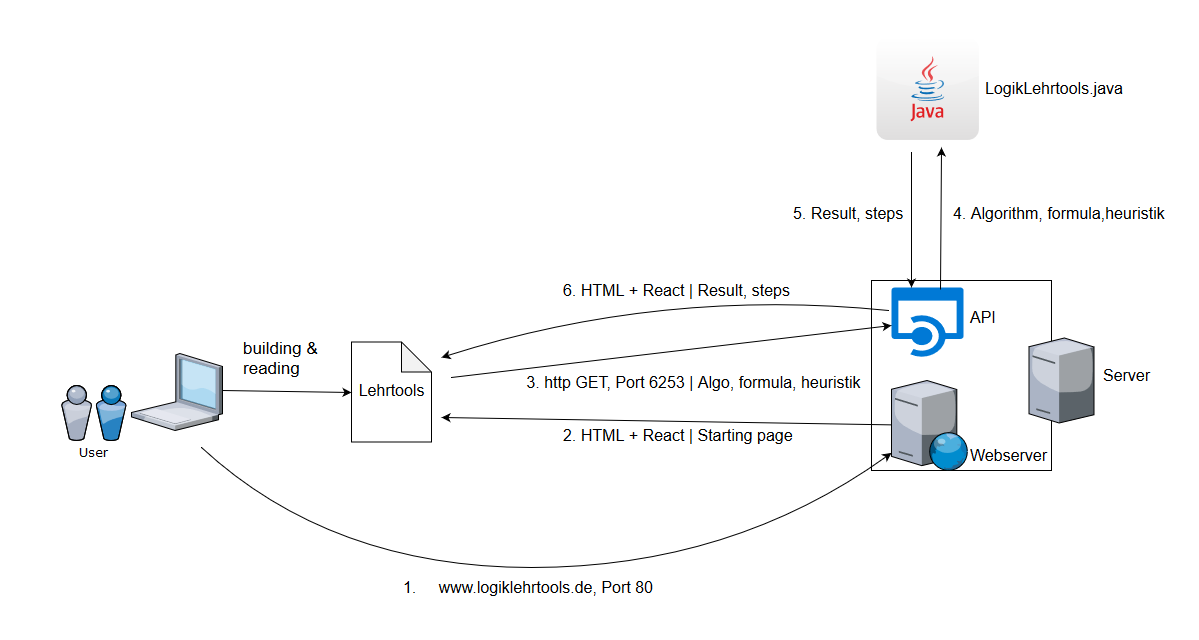
\includegraphics[width=15cm]{../Abbildungen/AblaufLehrtools.png}}
  \caption{Ablauf der Anwendung}
  \label{fig1_1}
\end{figure}
\section{Anpassung der Java Software}
Um das bereits vorliegende Java-Programm von Herrn Espinoza verwenden zu können waren einige Modifikationen daran notwendig. Herr Espinoza hatte seine Applikation mit Benutzeroberfläche entworfen und die logischen Abläufe an eine solche angepasst. Die Aktionen der Applikation wurden alleinig durch die Zustände und Nutzeraktionen dieser Benutzeroberfläche gesteuert. Während das für ein Standalone-Programm durchaus sinnvoll war, warf es Schwierigkeiten für die Webapplikation auf. Sind die Aktionen einer Webapplikation von früheren Aktionen oder Inputs abhängig, so ist  eine sehr viel größere Menge an Kommunikation zwischen Server und Client nötig, ebenso wie eine komplexere Benutzeroberfläche und ein höheres Maß an Handlungen der Nutzer. \\
Für dieses Projekt war eine stateless Implementation, also eine in der das Output nur vom Input und nicht von verschiedenen Zuständen abhängig ist besser geeignet. Da die Grundidee des Tools die Anwendung verschiedener Algorithmen war. Da die Anwendung und Darstellung der Algorithmen festen Regeln folgen, war eine eine Implementation, die dies widerspiegelt, eine passendere Wahl. \\
Einzelne Funktionen wie die Wahl der nächsten Resolutionsvariable zwischen einzelnen Schritten im gewählten Algorithmus und die Möglichkeit einen Schritt zurück zu gehen wurden daher entfernt. Stattdessen ist nun vor der Anwendung des Algorithmus die Angabe einer Heuristik möglich. So ist ebenfalls die Reihenfolge der Resolutionsvariablen frei wählbar, allerdings nur einmal vor Ausführung des Tools. Ist eine andere Reihenfolge gewünscht, muss der Algorithmus erneut mit einer anderen Heuristik gestartet werden. \\
Ebenso wurde die Wahl der Subsumption-Reihenfolge entfernt. Bisher konnte die Reihenfolge der beiden Möglichkeiten (forward und backward subsumption) gewählt werden. Da aber nach Ausübung einer von beiden stets die anderen zu folgen hatte und das Ergebnis nach Anwendung beider Varianten ohnehin dasselbe war, war diese Wahl unnötig. Stattdessen wird nun immer zuerst forward und dann backward subsumption durchgeführt. \\
Ebenso wurde die Auswahl der Eingabesyntax entfernt, da nicht zu erwarten ist, dass ein Nutzer verschiedene Eingabesprachen verwenden wird. Stattdessen scheint es wahrscheinlicher, dass sich Nutzer leichter an eine einzige Syntax gewöhnen um diese dann flüssig verwenden zu können.\\
Durch diese Anpassungen ist die Nutzerinteraktion des Tools auf wenige Schritte beschränkt. Der Nutzer kann lediglich seine Formel eingeben, optional eine Heuristik wählen und dann den gewünschten Algorithmus starten. Alle folgenden Schritte bis zur Anzeige des Resultats sind nicht beeinflussbar und daher immer gleich. Unter dem Ergebnis werden die einzelnen Schritte bis zur Lösung angezeigt. Diese Lösung mit weniger Interaktion konzentriert sich auf ein effizientes Angebot der Grundfunktionalität des Tools, ohne unnötige Wahlmöglichkeiten und bietet so besonders bei oftmaliger Nutzung große Zeitersparnis.\\
\begin{figure}[htb]
     \centerline{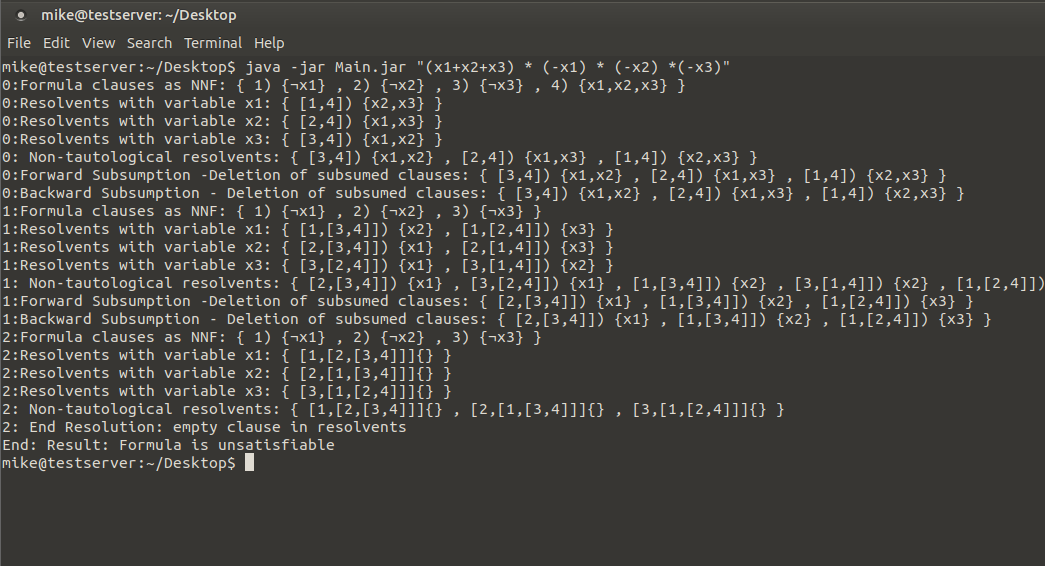
\includegraphics[width=14cm]{../Abbildungen/javaAusgabe.png}}
  \caption{Anwendung des Java-Programms mit Ausgabe}
  \label{fig1_1}
\end{figure}\\
Unabhängig von den Änderungen am logischen Ablauf wurde die Art des In- und Outputs ebenfalls abgewandelt. Das Tool liegt als jar-Datei auf dem Server und  arbeitet nun ausschließlich mit den Argumenten, die ihm bereits beim Start durch die API (siehe 5.4) übergeben werden. Danach werden keine zusätzlichen Parameter benötigt. \\
Die Teilschritte und das Endergebnis werden über die Kommandozeile ausgegeben, wo sie von der API gelesen und verarbeitet werden. In Abbilung 5.1 ist eine beispielhafte Anwendung des Java-Programms auf eine Formel zu sehen.\\

\section{Webserver}
Um die Webseite anzuzeigen wird sie über einen Webserver ausgegeben. Für dieses Projekt wurde ein Apache Webserver verwendet, es wäre aber problemlos möglich kleinere und ressourcenärmere Webserver zu implementieren. Der Webserver ist bei diesem Projekt von eher geringer Bedeutung, da React dynamische Webseiten erzeugt deren Inhalte nicht vom Server, sondern clientseitig berechnet werden. Der Server liefert lediglich den Programmiercode der Seiten, kann diesen jedoch selbst nicht oder nur teilweise interpretieren. \\
Aus diesem Grund sind für den Webserver in diesem Fall auch keine der üblichen Optimierungen notwendig. Sogar bei sehr großen Nutzerzahlen wird pro Anfrage nur ein sehr kleiner Aufwand entstehen. Da wie in 5.1 bereits erwähnt auch keine Zustände verwaltet werden müssen, besteht nur ein geringer Kommunikationsaufwand zwischen Nutzern und Server. Sogar bei Benutzung des Tools entsteht keinerlei Rechenaufwand für den Webserver, da die Berechnung der Ergebnisse von der API und dem Java Programm und die Anzeige der Ergebnisse wiederum von den Nutzergeräten erledigt wird. Pro Nutzer wird die Seite also nur einmal ausgeliefert und dann verwendet, bis die Seite neu geladen oder geschlossen wird.
\section{React Applikation}
Die React Applikation wurde mithilfe der-Toolchain Create React App erstellt. Wie bereits in Kapitel 4 ist diese ist für derartige single-page Apps besonders gut geeignet. Dank Create React App sind alle nötigen Abhängigkeiten und Ordnerstrukturen von Projektbeginn an gegeben. \\
Bei Aufruf der Seite wird die Eingabemaske angezeigt:\\
\begin{figure}[htb]
     \centerline{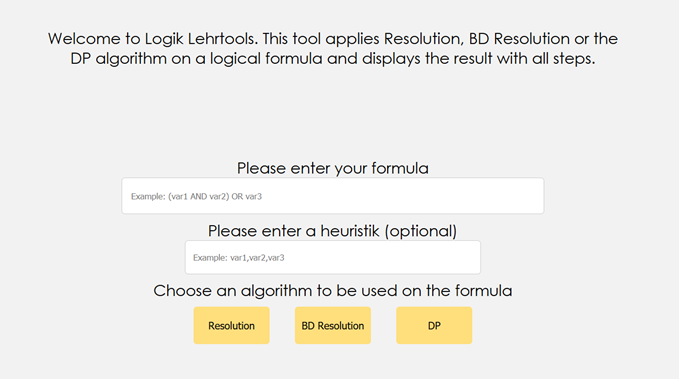
\includegraphics{../Abbildungen/eingabe.png}}
  \caption{Eingabemaske}
  \label{fig1_1}
\end{figure}\\
Dank JSX ähnelt der Code in React, beispielsweise für das Eingabefeld der Formel, dabei stark HTML:\\
\begin{figure}[htb]
     \centerline{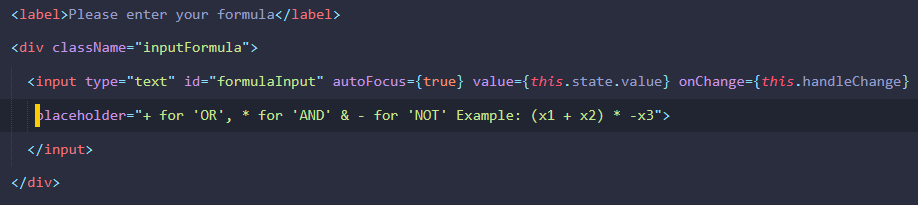
\includegraphics[width=14cm]{../Abbildungen/formulaInput.png}}
  \caption{Eingabefeld der Formel in JSX-Syntax}
  \label{fig1_1}
\end{figure}\\
Wie in Abbildung 5.3 zu erkennen ist, verfügt das Feld über einen Zustand 'this.state'. Dessen Wert wird bei Laden der Seite mit '', also leer, initialisiert. Die Funktion 'onChange', zu sehen in Abbildung 5.4, die diesem Komponenten hier unter anderem übergeben wird sorgt dafür, dass die vom Nutzer eingegebene Formel den neuen Wert von 'this.state.value' bildet, welcher gleichzeitig auch im Eingabefeld angezeigt wird.\\
\begin{figure}[htb]
     \centerline{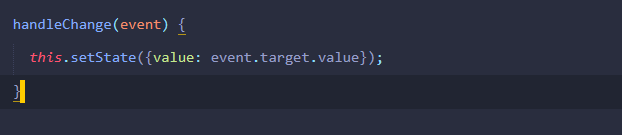
\includegraphics[width=14cm]{../Abbildungen/handleChange.png}}
  \caption{handleChange-Funktion}
  \label{fig1_1}
\end{figure}\\
Nachdem der User die Formel, eventuell eine Heuristik und den Algorithmus eingegeben hat, werden diese Angaben als Daten eines HTTP GET-Requests an den Server geschickt. Um diesen Request zu erzeugen wird Axios verwendet, ein schlanker und weit verbreiteter HTTP Client.
Dessen Installation und Nutzung ist dank der Modularität von React nur eine Sache von wenigen Zeilen. Nach Installation mittels eines Paketmanagers muss lediglich eine entsprechende Import-Zeile in der Javascript-Datei eingefügt werden. Anschließend kann der HTTP Client sofort mit allen Funktionen genutzt werden. \\
Als Ziel des GET-Requests wird ein anderer Port als der des Webservers verwendet, um die Daten an die Server API zu schicken. Die Daten werden im JSON-Format verschickt, da dieses von Axios unterstützt wird und die Daten von der API leicht ausgelesen werden können. In Abbildung 5.5 ist die Implementation am Beispiel Resolution dargestellt.
\begin{figure}[H]
     \centerline{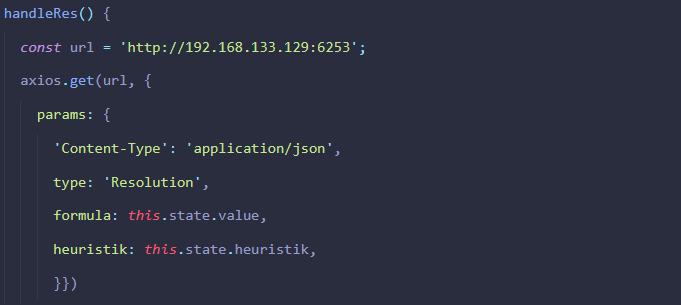
\includegraphics[width=14cm]{../Abbildungen/axiosResolution.png}}
  \caption{GET-Request für die Resolution}
  \label{fig1_1}
\end{figure}
Nach Berechnung der Ergebnisse erhält React eine Antwort mit diesen als HTML-Tabelle. Mit Hilfe der React-Funktion 'dangerouslySetInnerHTML' React ist in der Lage diesen HTML-Code ohne weiteres in den bestehenden Code einzugliedern. Der abschreckende Name dieser Funktion wurde gewählt, da es generell gefährlich sein kann Nutzerinput ohne weiteres darzustellen. An dieser Stelle besteht keine solche Gefahr, da dieses Input von Teilen der Projektarchitektur generiert wurde.
Sobald die Daten erhalten und mittels 'dangerouslySetInnerHTML' angezeigt werden, entsteht auf der Webseite die erhaltene Tabelle (siehe Abbildung 5.6).\\
Um das Ergebnis auch kompakt darzustellen, untersucht React mittels String-matching das erhaltene Ergebnis und gibt je nach Fall an ob die Formel erfüllbar ist oder nicht. Dazu wird Reacts Fähigkeit genutzt nicht nur HTML-Code, sondern sogar React-Code in Variablen speichern und direkt in bestehenden Code einbauen zu können. Die Methode, die das Ergebnis untersucht erstellt eine entsprechende React-Komponente und übergibt diesen an die passende Stelle im React-Code. \\
Um die Navigation für den Nutzer zu erleichtern, springt die Webseite nach dem Starten des Tools direkt an die Stelle, an der das Ergebnis angegeben wird. Dort gibt es durch einen entsprechenden Button die Möglichkeit zur Tabelle mit den Einzelschritten zu springen.
\begin{figure}[!htb]
     \centerline{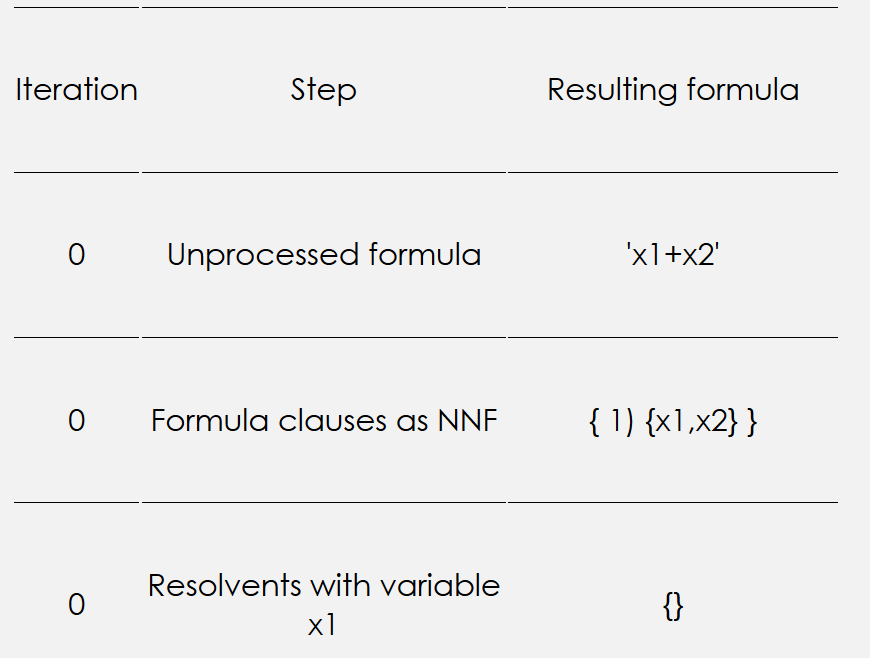
\includegraphics[width=14cm]{../Abbildungen/steps.png}}
  \caption{Ergebnistabelle}
  \label{fig1_1}
\end{figure}
\section{Server API}
Die API stellt die Schnittstelle zwischen Nutzereingabe und Java Applikation dar. Ihre Aufgaben sind das Empfangen der eingegebenen Daten, die Umwandlung dieser Daten in Startbefehle für die Applikation und das Senden der Ergebnisse, die von der Applikation ausgegeben werden. Häufige Lösungen für Anforderungen dieser Art beinhalten das Nutzen des Webservers als Proxy, der bestimmte Anfragen an ein Framework weiterleitet. Da aber in diesem Fall die Anzahl der möglichen Fälle sehr gering ist, bot sich eine direktere und schmalere Lösung an.\\
Die Schnittstelle wurde daher über ein Python-Skript realisiert. Dieses bedient sich des Python „BaseHTTPServer“ Moduls, welches einen sehr kleinen HTTP-Server erzeugt. Der Server ist in der Lage auf einem angegebenen Port auf HTTP-Requests zu warten, diese zu verarbeiten und angepasste Antworten zu senden. \\
Für dieses Projekt muss lediglich auf den GET-Request den React mittels Axios versendet gewartet werden. Es sind keinerlei andere Anfragen zu erwarten, weshalb Anfragen die nicht in das Muster passen sofort verworfen werden können.\\
Handelt es sich um den erwarteten Request, werden die beinhalteten Daten aus JSON geparst und in einen Kommandozeilenbefehl verarbeitet. Dieser Befehl startet die Java-Applikation mit den erhaltenen Parametern.\\
Wie bereits in 5.1 erwähnt erzeugt die Applikation Ausgaben für die Komandozeile. Diese werden im Skript aufgefangen und können so als Datenset verwendet werden. Da React in der Lage ist HTML Code zu empfangen und direkt zu verwenden, kann an dieser Stelle ein weiteres Verpacken der Daten in JSON vermieden werden. Stattdessen wird eine Tabelle aufgebaut, in der die Ergebnisse strukturiert und übersichtlich präsentiert werden können. Der HTML-Code wird nicht mit dem Typ 'text/html', wie möglicherweise zu erwarten wäre, versehen. Stattdessen wird als Typ 'text/plain' angegeben. Grund dafür ist, dass so keine Notwendigkeit besteht, eine komplette HTML-Struktur aufzubauen. So ist es möglich nur den Code für die Tabelle zu senden, so dass er von der React Applikation ohne weiteres in die bereits bestehende Seite eingegliedert wird.


\clearpage

%%%%%%%%%%%%%%%%%%%%%%%%%%%%%%%%%%%%%%%%%%%%%%%%%%%%%%%%%%%%%%%%%%%%%%%%%%%%%
%%% Bibliographie
%%%%%%%%%%%%%%%%%%%%%%%%%%%%%%%%%%%%%%%%%%%%%%%%%%%%%%%%%%%%%%%%%%%%%%%%%%%%%

\addcontentsline{toc}{chapter}{Literaturverzeichnis}

\bibliographystyle{alpha}
\begin{thebibliography}{9}

  \bibitem{1}
  \textsc{Blog der React Entwickler, Artikel von Pete Hunt}\\
  \textit{Why did we build React?}\\
  \href{https://reactjs.org/blog/2013/06/05/why-react.html}{https://reactjs.org/blog/2013/06/05/why-react.html}\\
  Aufgerufen am 10.03.2019

  \bibitem{2}
  \textsc{Cory Gackenheimer}\\
  \textit{Introduction to React}\\
  \textsc{Appress Media LLC, 2015}\\
  \href{https://books.google.de/books?hl=de&lr=&id=NZCKCgAAQBAJ&oi=fnd&pg=PR6&dq=react+javascript&ots=KAvyPmyx-e&sig=vmxw0RuGUAADmEc_vZTL4VakTnE#v=onepage&q=react%20javascript&f=false}{Google Books Link}

  \bibitem{3}
  \textsc{Artikel von Paul Kögel}\\
  \textit{Motivation hinter React}\\
  \href{https://reactjs.de/artikel/react-tutorial-deutsch/#motivation-hinter-react}{https://reactjs.de/artikel/react-tutorial-deutsch/\#motivation-hinter-react}\\
  Aufgerufen am 10.03.2019

  \bibitem{4}
  \textsc{Artemij Fedosejev}\\
  \textit{React.js Essentials}\\
  \textsc{Packt Publishing, 2015}\\
  \href{https://books.google.de/books?hl=de&lr=&id=Rhl1CgAAQBAJ&oi=fnd&pg=PP1&dq=react+javascript&ots=JjvymzwSMG&sig=V3PsDnRjBuwxrtUaRyrYVkB6Ffk#v=onepage&q=react%20javascript&f=false}{Link zu Google Books Version}

  \bibitem{5}
  \textsc{Naimul Islam Naim}\\
  \textit{ReactJS:  An  Open  Source  JavaScript  Library for Front-end Developement}\\
  \textsc{Metropolia University of Applied Sciences, 2017}\\
  \href{https://www.theseus.fi/bitstream/handle/10024/130495/FInal_Year_Thesis.pdf}{https://www.theseus.fi/bitstream/handle/10024/130495/FInal\_Year\_Thesis.pdf}

  \bibitem{6}
  \textsc{Alex Banks and Eve Porcello}, \\
  \textit{Learning React}\\
  \textsc{O’Reilly Media, Inc., 2017}\\
  \href{http://www.r-5.org/files/books/computers/languages/escss/w-tkt/react/Alex_Banks_and_Eve_Porcello-Learning_React-EN.pdf}{http://www.r-5.org/files/books/computers/languages/escss/w-tkt/react/Alex\_Banks\_and\_Eve\_Porcello-Learning\_React-EN.pdf}
  \bibitem{7}
  \textsc{Artikel von Gianluca Guarini}\\
  \textit{Things nobody will tell you about React.js}\\
  \href{https://medium.com/@gianluca.guarini/things-nobody-will-tell-you-about-react-js-3a373c1b03b4}{https://medium.com/@gianluca.guarini/things-nobody-will-tell-you-about-react-js-3a373c1b03b4}\\
  Aufgerufen am 10.03.2019

  \bibitem{8}
  \textsc{Guide der Vue Entwickler}\\
  \textit{Comparison with Other Frameworks}\\
  \href{https://vuejs.org/v2/guide/comparison.html}{https://vuejs.org/v2/guide/comparison.html}\\
  Aufgerufen am 10.03.2019

  \bibitem{9}
  \textsc{Vorstellung von Preact}\\
  \textit{Eine Bibliothek der anderen Art.}\\
  \href{https://preactjs.com/}{https://preactjs.com/}\\
  Aufgerufen am 10.03.2019

  \bibitem{10}
  \textsc{Vorstellung von Riot}\\
  \textit{Riot vs React \& Polymer}\\
  \href{https://riot.js.org/v2/compare/}{https://riot.js.org/v2/compare/}\\
  Aufgerufen am 10.03.2019

  \bibitem{11}
  \textsc{React Dokumentation}\\
  \textit{Create a New React App}\\
  \href{https://reactjs.org/docs/create-a-new-react-app.html}{https://reactjs.org/docs/create-a-new-react-app.html}\\
  Aufgerufen am 10.03.2019

  \bibitem{12}
  \textsc{React Dokumentation}\\
  \textit{Add React to a Website}\\
  \href{https://reactjs.org/docs/add-react-to-a-website.html}{https://reactjs.org/docs/add-react-to-a-website.html}
  Aufgerufen am 10.03.2019

  \bibitem{eig}
  Alle Abbildung außer die nachfolgend aufgeführten:\\
  \textsc{Eigene Abbildung}

  \bibitem{Abb2.1}
  Abbildung 2.1:\\
  \textsc{CronJ-Artikel von Akash Bhandwalkar}\\
  \textit{Virtual Dom|Browser DOM what are these in React Js?}\\
  \href{https://www.cronj.com/blog/virtual-dom-react-js/}{https://www.cronj.com/blog/virtual-dom-react-js/}\\
  Aufgerufen am 10.03.2019

  \bibitem{Abb2.8}
  Abbildung 2.8:\\
  \textsc{Google-Trend Analyse: Vergleich von React, Angular und Vue}\\
  \href{https://trends.google.de/trends/explore?cat=31&date=today%205-y&q=react,angular,vue}{https://trends.google.de/trends/explore?cat=31\&date=today\%205-y\&q=react,angular,vue}\\
  Aufgerufen am 10.03.2019

  \bibitem{Abb3.5}
  Abbildung 3.5:\\
  \textsc{React Developer Tools}\\
  \href{https://chrome.google.com/webstore/detail/react-developer-tools/fmkadmapgofadopljbjfkapdkoienihi?hl=de}{https://chrome.google.com/webstore/detail/react-developer-tools/fmkadmapgofadopljbjfkapdkoienihi?hl=de}\\
  Aufgerufen am 10.03.2019


\end{thebibliography}



\clearpage

%%%%%%%%%%%%%%%%%%%%%%%%%%%%%%%%%%%%%%%%%%%%%%%%%%%%%%%%%%%%%%%%%%%%%%%%%%%%%
%%% Erklaerung
%%%%%%%%%%%%%%%%%%%%%%%%%%%%%%%%%%%%%%%%%%%%%%%%%%%%%%%%%%%%%%%%%%%%%%%%%%%%%
\thispagestyle{empty}
\section*{Selbst\"andigkeitserkl\"arung}

Hiermit versichere ich, dass ich die vorliegende Bachelorarbeit 
selbst\"andig und nur mit den angegebenen Hilfsmitteln angefertigt habe und dass alle Stellen, die dem Wortlaut oder dem 
Sinne nach anderen Werken entnommen sind, durch Angaben von Quellen als 
Entlehnung kenntlich gemacht worden sind. 
Diese Bachelorarbeit wurde in gleicher oder \"ahnlicher Form in keinem anderen 
Studiengang als Pr\"ufungsleistung vorgelegt. 

\vskip 3cm

Ort, Datum	\hfill Unterschrift \hfill 

\end{document}

